\chapter*{Planificación del proyecto}
En los primeros años del desarrollo de software, este se creaba sin seguir ningun enfoque formal. Muchos de los proyectos que se iniciaban terminaban fracasando por los retrasos en la entrega, el mal funcionamiento del producto o por no cumplir los requisitos del cliente. Además, la complejidad requerida en el software iba aumentando con el tiempo. 

Por ello, era necesario crear un marco que permitiera metodizar el desarrollo. Es así como surge la Ingeniería del Software, que acompaña al software durante todo su ciclo vital.

En nuestro proyecto vamos a aplicar este enfoque a la hora de desarrollar el producto, y en este apartado vamos a describir información general sobre su gestión, la metodología de desarrollo a seguir y otra información relativa a costes, riesgos y otros factores que influyen sobre el proyecto para asegurarnos de que se consiguen los objetivos en el tiempo previsto, detectando posibles amenazas y problemas a tiempo.

\section*{Gestión del proyecto}

\section*{Metodología de desarrollo}

Las metodologías se pueden clasificar en dos grandes bloques \cite{metodologiasDesarrollo}, tradicionales y ágiles. Las tradicionales son las que primero surgieron, se caracterizan por definir rígidamente los requisitos al inicio del proyecto. En ellas, se aplica una serie de etapas de forma lineal, y una vez alcanzada una de ellas no se puede volver atrás. Por todo esto no se adaptan bien a los cambios.

En general, los proyectos de software tienden a ser cada vez más complejos. Las metodologías ágiles surgieron con el objetivo de hacer los proyectos de desarrollo más dinámicos, de forma que se adaptaran mejor al entorno y a los cambios. Se basan en una metodología incremental, donde se van construyendo prototipos del producto poco a poco, añadiendo funcionalidades hasta obtener la aplicación final. Los equipos se reunen cada poco tiempo para intercambiar ideas y repartir las tareas a realizar.

A la hora de elegir la metodología que vamos a usar, debemos tener en cuenta los siguientes factores relativos a su naturaleza:

\begin{itemize}
    \item Se trata de un proyecto de investigación, donde vamos a aplicar diferentes técnicas de Aprendizaje Automático a la resolución de un problema. Por tanto, a priori no se conoce la calidad de los resultados que se van a obtener y el número de experimentos que va a ser necesario realizar.
    \item La intervención del experto en química va a ser fundamental durante el desarrollo del proyecto. Aportará información y feedback esencial durante todas las fases.
\end{itemize}

Por estas razones, creemos que la metodología de desarrollo que mejor se adapta a nuestras necesidades es una metodología ágil, ya que nos provee de gran flexibilidad, permitiendo el desarrollo del proyecto de una forma incremental donde obtenemos feedback del cliente y del experto en cada iteración.

Revisando las distintas metodologías \cite{despa2014comparative}, creemos que una buena candidata es SCRUM \cite{schwaber1997scrum}: es posiblemente una de las más utilizadas en la actualidad, y los proyectos que la utilizan cuentan con las siguientes características:

\begin{itemize}
    \item \textbf{Entregable flexible:} Su contenido viene dado por lo que demanda el entorno. 
    \item \textbf{Calendario flexible:} El entregable puede ser requerido antes o después de lo previsto.
    \item \textbf{Equipos pequeños:} Los equipos están formados por pocas personas, de forma que la comunicación y sincronización entre sus miembros es alta. 
    \item \textbf{Revisiones frecuentes:} El progreso del equipo se evalúa de forma periódica y frecuentemente, de forma que se ponen en común las dificultades encontradas y se intentan resolver con la ayuda de todos los miembros.
    \item \textbf{Colaboración:} La colaboración entre todos los miembros del equipo es muy alta, así como entre el equipo y entidades externas como el cliente.
\end{itemize}

Cuando se trabaja con esta metodología en un equipo existe un miembro conocido como SCRUM manager. Es el encargado de guiar al equipo en el desarrollo y en la aplicación de la metodología. Aún así, en SCRUM el equipo es muy importante y todos sus miembros participan con su opinión. Esta metodología consta de las siguientes fases:

% TODO: Si fuera necesario, añadir información sobre los tipos de equipos. En el paper de SCRUM aparece información sobre estos.

\begin{figure}[H]
    \centering
        \fbox{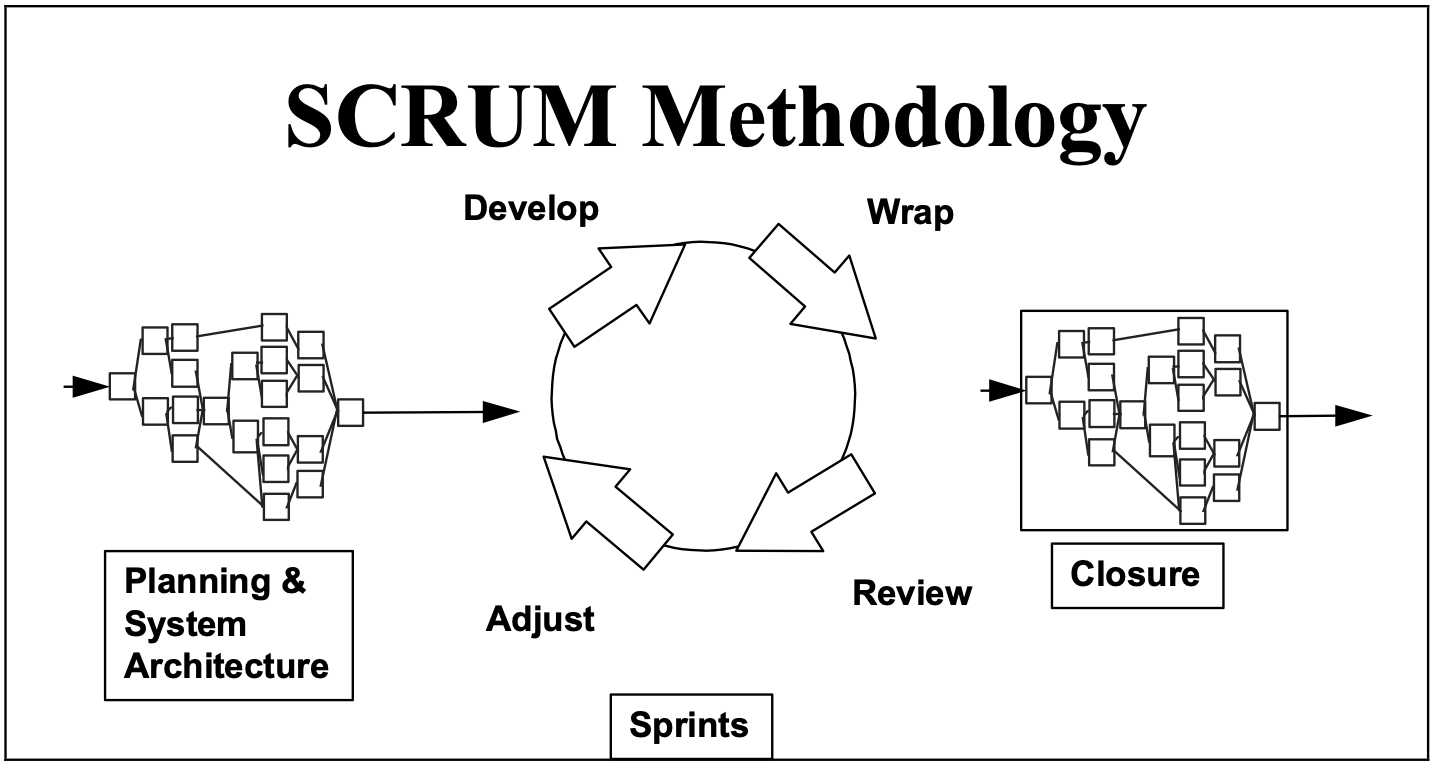
\includegraphics[scale=0.45]{imagenes/scrum.png}}  
        \caption{Fases de la metodología SCRUM \cite{schwaber1997scrum}} \label{fig:figura1}
    \end{figure}

\begin{itemize}
    \item \textbf{Pregame:} 
    \begin{itemize}
        \item \textit{Planificación:} En esta fase se crea la lista de tareas a realizar (backlog list), se fija la fecha de entrega del producto y su funcionalidad, se forma el equipo (o equipos) de trabajo, se valoran los riesgos que puedan surgir, los costes y finalmente se revisa todo y se aprueba el proyecto.
        \item \textit{Arquitectura/Diseño de alto nivel:} Se revisan los elementos en el backlog, se realizan cambios si es necesario para poder implementarlos, se perfila la arquitectura del sistema teniendo en cuenta estos cambios y una reunión es organizada para revisar el diseño, donde cada equipo presenta una propuesta para implementar cada backlog.
    \end{itemize}
    \item \textbf{Game:} Corresponde con el conocido Sprint de la metodología SCRUM. Es la parte iterativa de la metodología, que se ejecuta varias veces hasta conseguir el producto final y está formada por las siguientes subtareas:
    \begin{itemize}
        \item \textit{Desarrollo:} Lo primero que se realiza es definir los cambios que hay que realizar en los backlogs para poder implementarlos. Se dividen las tareas presentes en el backlog en paquetes, y se completan estos paquetes diseñando, desarrollando, implementando, testeando y documentando los cambios.
        \item \textit{Envoltura:} Se cierran los paquetes, creando una ejecutable que incorpora los cambios y se explica como cumplen lo especificado en los backlogs.
        \item \textit{Revisión:} Todos los equipos se reunen para presentar el trabajo. El desarrollo obtenido se evalúa y se añaden nuevas tareas que puedan surgir al backlog. Se evalúa el riesgo y se realizan propuestas en base a este.
        \item \textit{Ajuste:} Se consolida la información recibida durante la revisión.
    \end{itemize}
    
    \item \textbf{Postgame:}
    \begin{itemize}
        \item \textit{Cierre:} Cuando el gestor del proyecto considera que el producto está terminado y cumple con los requisitos solicitados por el cliente se entra en esta fase, donde se prepara el producto para su despliegue. Integración, generación de la documentación, testeo y marketing son algunas de las actividades que se realizan en este paso.
    \end{itemize}

\end{itemize}

Estas características que hemos mencionado son las especificadas en la definición original de SCRUM. Aún así, en la práctica cada proyecto las adapta a sus necesidades. En general, los sprints suelen tener una duración de 2 o 3 semanas. En nuestro caso tendrán 1 o 2 semanas de duración.

